\onehalfspaced

\begin{algorithm}[h!]
\caption{}\label{modelselection}
\textbf{Input}: $\delta$, the allowable deviation from the expected upper bound on BLEU score (using all redundant translations); $\alpha$, the upper bound BLEU score; a training set $S = \{\vec f^{s}_{i,j},y^{s}_{i,j})_{i=1..n}^{j=1..4}\}$ and a validation set $V = \{(\vec f^{v}_{i,j},y^{v}_{i,j})_{i=1..n}^{j=1..4}\}$ where $\vec f_{i,j}$ is the feature vector for $t_{i,j}$ which is the $jth$ translation of the source sentence $s_{i}$ and $y_{i,j}$ is the label for $\vec f_{i,j}$.\\
\textbf{Output}: $\theta$, the threshold between acceptable and unacceptable translations; $\vec{w}$, a linear regression model parameter. 
\begin{algorithmic}[1]
\State \textbf{initialize} $\theta \leftarrow 0$,$\vec{w}\leftarrow \emptyset$ 
\State $\vec{w'}\leftarrow$ train a linear regression model on $S$
\State $maxbleu \leftarrow$ select best translations for each $s_i \in S$ based on the model parameter $\vec{w'}$ and record the highest model predicted BLEU score
\While {$\theta \neq maxbleu $} 
\For {$i \leftarrow 1$ to $n$}
\For {$j \leftarrow 1$ to $4$}
\If {$\vec{w'}\cdot \vec f^v_{i,j} > \theta \wedge j < 4 $}
             select $t^{v}_{i,j}$ for $s_i$ and \textbf{break}
\EndIf
\If {$ j == 4 $} select $t^{v}_{i,j}$ for $s_i$
\EndIf
\EndFor
\EndFor
\State $q \leftarrow$ calculate translation quality for V
\If {$q > \delta \cdot \alpha$} \textbf{break}
\Else \text{  } $\theta = \theta + stepsize$
\EndIf
\EndWhile
\State $\vec {w} \leftarrow$ train a linear regression model on $S \cup V$
\State \textbf{Return}: $\theta$ and model parameter $\vec{w}$
%\EndProcedure
\end{algorithmic}
\end{algorithm}



\section{Reducing the Number of Translations}
The first mechanism that we introduce to optimize cost is one that reduces the number of translations.  Our goal is to recognize when we have got a good translation of a source sentence and to immediately stop purchasing additional  translations of that sentence.  The crux of this method is to decide whether a translation  is `good enough,' in which case we do not gain any benefit from  paying for another redundant translation.  

Our translation reduction method allows us to set an empirical definition of `good enough'.  
We define an oracle upper bound $\alpha$ to be the estimated BLEU score using the full set of non-professional translations.
We introduce a parameter $\delta$ to set how much degradation in translation quality is allowable.  For instance, we may fix $\delta$ at 95\%, meaning that the resulted BLEU score should not drop below 95\% of the $\alpha$ after reducing the number of translations.   We train a model to search for a threshold $\theta$ between acceptable and unacceptable translations for a specific value of $\delta$. 

For a new translation, our model scores it, and if its score is higher than $\theta$, then we do not solicit another translation. Otherwise, we continue to solicit translations.  Algorithm \ref{modelselection} details the process of model training and searching for $\theta$. 


 \begin{table}
 \center
\begin{tabular}{c|c|c}
\hline
$\delta$(\%) & BLEU Score & \# Trans. \\ \hhline{===}
90    & 36.26      & 1.63            \\
91    & 36.66      & 1.69             \\
92    & 36.93      & 1.78             \\
93    & 37.23      & 1.85             \\
94    & 37.48      & 1.93             \\
95    & 38.05      & 2.21             \\
96    & 38.16      & 2.30             \\
97    & 38.48      & 2.47             \\
98    & 38.67      & 2.59             \\
99    & 38.95      & 2.78             \\
100   & 39.54      & 3.18             \\ \hline
\end{tabular}
\caption{The relation among the $\delta$ (the allowable deviation from the expected upper bound on BLEU score), the BLEU score for translations selected by models from partial sets and the averaged size of translation candidates set for each source sentence (\textit{\# Trans}).  }
    \label{orderanother}
\end{table}


\subsection{Experiment}
 We divide data into a training set (10\%), a validation set (10\%) and a test set (80\%). 
We use the validation set to search for $\theta$. The upper bound BLEU is set to be 40.13 empirically as the oracle upper bound. 
We then vary the value of $\delta$ from 90\% to 100\%, and sweep values of $\theta$ by incrementing it in step sizes of 0.01.
We report results based on a five-fold cross validation, rotating the training, validation and test sets.

\subsubsection{Baseline and upper bound} 
The baseline selection method of randomly picking one translation for each source sentence achieves a BLEU score of 29.56. To establish an upper bound on translation quality, we perform an oracle experiment selects best translation for each source segment.  It reaches a BLEU score of 40.13.

\subsubsection{Translation reducing method} 

Table \ref{orderanother} shows the results for translation reducing method.  The $\delta$ variable correctly predicts the deviation in BLEU score when compared to using the full set of translations.   If we set $\delta$ $<$0.95 then we lose 2 BLEU points, but we cut the cost of translations in half, since we pay for only two translations of each source segment on average.


\begin{figure}
  \centering
  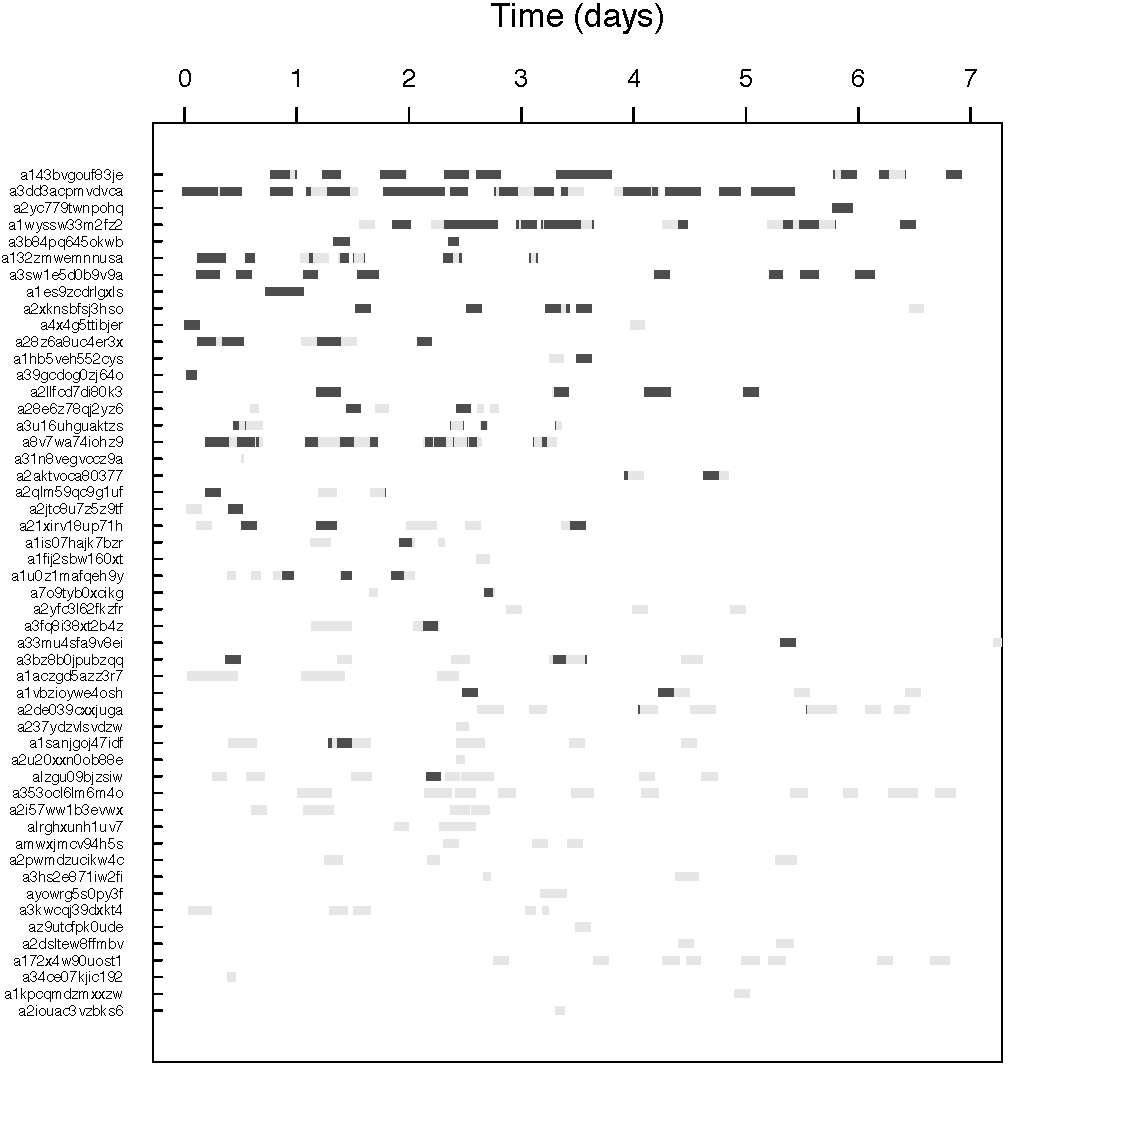
\includegraphics[width=\linewidth]{WorkerPerf/wp.pdf}
  \caption{A time-series plot of all of the translations produced by Turkers (identified by their WorkerID serial number). Turkers are sorted with the best translator at the top of the y-axis. Each tick represent a single translation and dark color means better than average quality.
}
    \label{fworkerperf}
\end{figure}
